\documentclass{article}
\usepackage[utf8]{inputenc}
\usepackage{amsmath}
\usepackage{amsfonts}
\usepackage{amssymb} % Añadido para asegurar soporte completo de símbolos matemáticos
\usepackage{tikz}

\begin{document}

El grafo de Cayley presentado para el grupo diédrico $D_4$ es matemáticamente correcto y modela con total precisión la estructura del grupo de simetrías de un cuadrado (de orden 8). A continuación se desglosa la verificación formal de cada uno de sus componentes basados en la presentación algebraica:

\[
D_4 = \langle r, f \mid r^4 = e, \, f^2 = e, \, fr = r^{-1}f \rangle
\]

\section{Definición de los Generadores y Relaciones}
\begin{itemize}
    \item \textbf{Rotación ($r^4 = e$):} Representa una rotación de $90^\circ$ en sentido horario. Aplicarla cuatro veces consecutivas regresa el sistema al estado de identidad ($e$).
    \item \textbf{Reflexión ($f^2 = e$):} Representa una simetría axial. Al ser un operador involutivo, aplicarlo dos veces consecutivas anula su efecto ($f \cdot f = e$).
    \item \textbf{Relación no abeliana ($fr = r^{-1}f$ o $fr = r^3f$):} Esta relación define la interacción no conmutativa entre rotaciones y reflexiones. Como el orden de $r$ es 4, se tiene que $r^{-1} = r^3$.
\end{itemize}

\section{Análisis de las Órbitas en el Grafo}

\subsection{El Ciclo Exterior (Rotaciones Puras, Camino Verde-Azul)}
La acción de la rotación se define multiplicando por la derecha por el generador $r$ (es decir, la transición es de la forma $x \xrightarrow{\cdot r} xr$). 
Para los elementos sin reflexión (ciclo exterior), el avance sigue un sentido horario estándar:
\[
e \xrightarrow{\cdot r} r \xrightarrow{\cdot r} r^2 \xrightarrow{\cdot r} r^3 \xrightarrow{\cdot r} e
\]
Esto coincide perfectamente con las flechas exteriores continuas de color azul-verde.

\subsection{El Ciclo Interior (Elementos Reflejados)}
Al multiplicar por la derecha por $r$ a un elemento que ya posee una componente de reflexión ($xf \xrightarrow{\cdot r} xfr$), la relación $fr = r^3f$ altera el sentido de la rotación:
\begin{itemize}
    \item \textbf{Partiendo de $f$:} 
    \[ f \cdot r = r^3f \]
    La flecha dirigida va desde el nodo $f$ hasta el nodo $r^3f$.
    
    \item \textbf{Partiendo de $r^3f$:} 
    \[ r^3f \cdot r = r^3(fr) = r^3(r^3f) = r^6f = r^2f \]
    La flecha va desde $r^3f$ hasta $r^2f$ (ya que $r^4 = e$, por lo que $r^6 = r^2$).
    
    \item \textbf{Partiendo de $r^2f$:} 
    \[ r^2f \cdot r = r^2(fr) = r^2(r^3f) = r^5f = rf \]
    La flecha va desde $r^2f$ hasta $rf$ (dado que $r^5 = r$).
    
    \item \textbf{Partiendo de $rf$:} 
    \[ rf \cdot r = r(fr) = r(r^3f) = r^4f = f \]
    La flecha va desde $rf$ hasta $f$.
\end{itemize}

Esta secuencia matemática genera el ciclo interno:
\[
f \xrightarrow{\cdot r} r^3f \xrightarrow{\cdot r} r^2f \xrightarrow{\cdot r} rf \xrightarrow{\cdot r} f
\]
El cual se desplaza de forma \textbf{antihoraria}, ilustrando visualmente cómo la reflexión invierte la orientación del plano.

\subsection{Los Puentes de Reflexión (Camino Naranja Punteado)}
Las aristas punteadas representan la multiplicación por la derecha por el generador $f$ ($x \xrightarrow{\cdot f} xf$). Dado que $f$ es una involución ($f^2 = e$), estas conexiones son bidireccionales, actuando como puentes de doble sentido entre los ciclos interior y exterior:
\begin{align*}
    e \cdot f = f &\iff f \cdot f = e \\
    r \cdot f = rf &\iff rf \cdot f = r \\
    r^2 \cdot f = r^2f &\iff r^2f \cdot f = r^2 \\
    r^3 \cdot f = r^3f &\iff r^3f \cdot f = r^3
\end{align*}
El grafo plasma con absoluta fidelidad estos pares de conexiones simétricas mediante los puentes naranjas.

\section{Conclusión}
El grafo de Cayley para $D_4$ cumple de manera rigurosa con la estructura del grupo algebraico. Representa tanto el carácter no abeliano como las propiedades geométricas de simetría de forma clara y formal.

\begin{figure}[htbp]
\centering
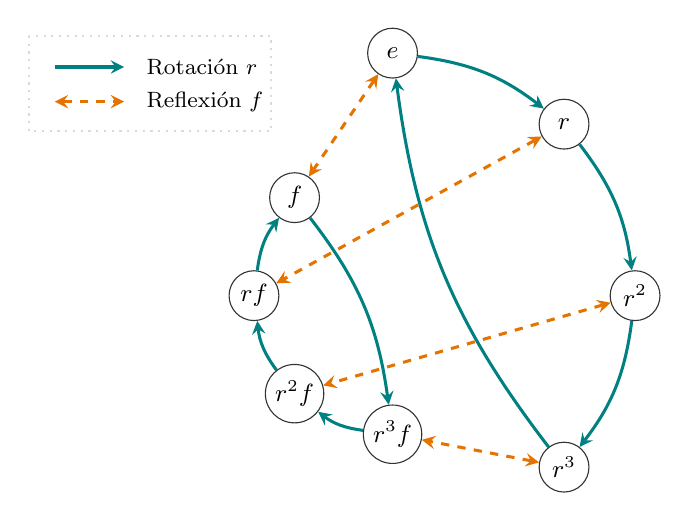
\begin{tikzpicture}[
    scale=2.2,
    % Estilo profesional para los nodos (elementos del grupo)
    nodo/.style={circle, draw=black!80, fill=white, inner sep=1.5pt, minimum size=1.8em, font=\small},
    % Estilos fijos para las aristas (generadores) con flechas elegantes
    flechaRotacion/.style={->, >=stealth, thick, color=teal, line width=1.1pt},
    flechaReflexion/.style={<->, >=stealth, thick, color=orange!90!black, dashed, line width=1.1pt}
]

    % --- DEFINICIÓN DE LOS 8 VÉRTICES (Distribución angular en un octágono) ---
    % Rotaciones (Círculo exterior)
    \node[nodo] (e)   at (90:1.4)   {$e$};
    \node[nodo] (r)   at (45:1.4)   {$r$};
    \node[nodo] (r2)  at (0:1.4)    {$r^2$};
    \node[nodo] (r3)  at (315:1.4)  {$r^3$};
    
    % Reflexiones combinadas (Círculo interior para evitar cruces)
    \node[nodo] (f)   at (135:0.8)  {$f$};
    \node[nodo] (rf)  at (180:0.8)  {$rf$};
    \node[nodo] (r2f) at (225:0.8)  {$r^2f$};
    \node[nodo] (r3f) at (270:0.8)  {$r^3f$};


    % --- ARISTAS DEL GENERADOR 'r' (Acción por la derecha g -> g*r) ---
    % Ciclo exterior: e -> r -> r^2 -> r^3 -> e
    \draw[flechaRotacion] (e) to[bend left=15] (r);
    \draw[flechaRotacion] (r) to[bend left=15] (r2);
    \draw[flechaRotacion] (r2) to[bend left=15] (r3);
    \draw[flechaRotacion] (r3) to[bend left=15] (e);

    % Ciclo interior: f -> r^3f -> r^2f -> rf -> f
    % (inversión causada por fr = r^{-1}f)
    \draw[flechaRotacion] (f) to[bend left=15] (r3f);
    \draw[flechaRotacion] (r3f) to[bend left=15] (r2f);
    \draw[flechaRotacion] (r2f) to[bend left=15] (rf);
    \draw[flechaRotacion] (rf) to[bend left=15] (f);


    % --- ARISTAS DEL GENERADOR 'f' (Reflexión: Involución bidireccional) ---
    % f^2 = e, por lo que cada conexión es una involución
    \draw[flechaReflexion] (e) -- (f);
    \draw[flechaReflexion] (r) -- (rf);
    \draw[flechaReflexion] (r2) -- (r2f);
    \draw[flechaReflexion] (r3) -- (r3f);


    % --- LEYENDA INTEGRADA DE NIVEL EDITORIAL ---
    \begin{scope}[shift={(-2.1,1.5)}]
        \draw[fill=white, draw=gray!30, dotted, thick] (0,0) rectangle (1.4,-0.55);
        \draw[flechaRotacion, ->] (0.15,-0.18) -- (0.55,-0.18) node[right, black, font=\footnotesize] {\, Rotación $r$};
        \draw[flechaReflexion, <->] (0.15,-0.38) -- (0.55,-0.38) node[right, black, font=\footnotesize] {\, Reflexión $f$};
    \end{scope}

\end{tikzpicture}
\caption{Grafo de Cayley del grupo diédrico $D_4 = \langle r, f \mid r^4 = e, f^2 = e, fr = r^{-1}f \rangle$. El ciclo exterior azul-verde representa las rotaciones puras del cuadrado, mientras que el ciclo interior refleja la inversión inducida por la relación no abeliana $fr=r^{-1}f$. Los puentes naranjas representan la acción involutiva de la reflexión.}
\label{fig:cayley_d4}
\end{figure}

\end{document}
